\begin{figure}[!ht]
    \centering
    \subfloat[Labyrinth]{
        \label{Labyrinth}
        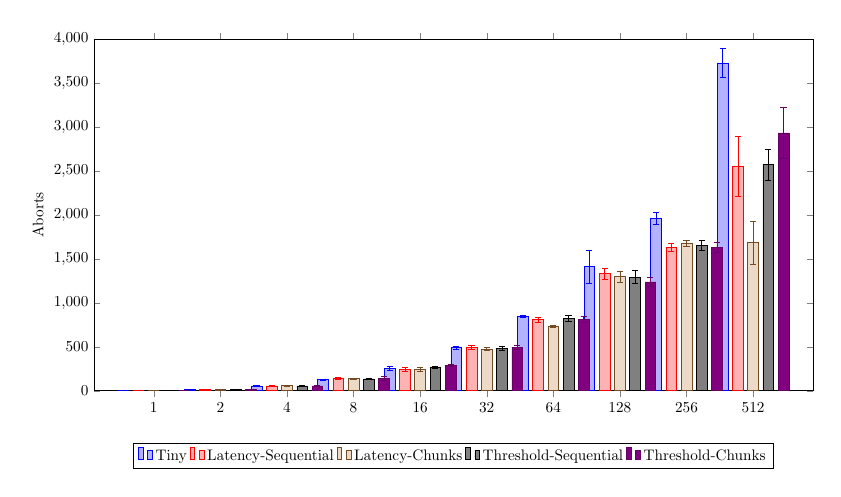
\begin{tikzpicture}[scale=0.55, baseline]
        \begin{axis}[
            width=1.5 \linewidth,
            height=0.8 \linewidth,
            %media de tempo intruder
            ybar=3pt,
            %enlargelimits=0.10,
            legend style={at={(0.5,-0.15)}, anchor=north, legend columns=-1},
            ylabel=Aborts,
            symbolic x coords={1, 2, 4, 8, 16, 32, 64, 128, 256, 512},
            xtick=data,
            ymin=0,
            ymax=4000,
            bar width=7pt,
            % nodes near coords,
            nodes near coords align={vertical},
        ]
        \addplot+[error bars,y dir=both, y explicit] coordinates {
            (1,0.0)+-(1,0.0) (2,12.2)+-(2,2.63) (4,53.2)+-(4,5.94) (8,127.2)+-(8,6.14) (16,258.0)+-(16,24.04) (32,490.2)+-(32,16.41) (64,847.0)+-(64,12.39) (128,1413.4)+-(128,186.85) (256,1959.6)+-(256,67.08) (512,3727.2)+-(512,167.11) 
        };
        \addplot+[error bars,y dir=both, y explicit] coordinates {
            (1,0.0)+-(1,0.0) (2,11.4)+-(2,0.48) (4,56.0)+-(4,4.09) (8,142.0)+-(8,12.85) (16,245.8)+-(16,19.87) (32,491.2)+-(32,25.11) (64,811.8)+-(64,28.18) (128,1334.2)+-(128,63.09) (256,1633.4)+-(256,41.57) (512,2556.6)+-(512,340.72)
        };
        \addplot+[error bars,y dir=both, y explicit] coordinates {
             (1,0.0)+-(1,0.0) (2,12.2)+-(2,1.46) (4,56.4)+-(4,3.61) (8,136.4)+-(8,10.30) (16,245.4)+-(16,19.39) (32,473.2)+-(32,16.47) (64,734.8)+-(64,11.12) (128,1298.4)+-(128,60.09) (256,1677.2)+-(256,35.19) (512,1686.8)+-(512,244.04)
        };
        \addplot+[error bars,y dir=both, y explicit] coordinates {
            (1,0.0)+-(1,0.0) (2,11.8)+-(2,0.97) (4,54.8)+-(4,2.78) (8,134.8)+-(8,4.39) (16,271.2)+-(16,11.35) (32,482.8)+-(32,22.57) (64,822.0)+-(64,36.78) (128,1291.2)+-(128,74.59) (256,1657.8)+-(256,58.13) (512,2571.6)+-(512,174.36)
        };
        \addplot+[error bars,y dir=both, y explicit] coordinates {
            (1,0.0)+-(1,0.0) (2,11.0)+-(2,1.2) (4,55.72)+-(4,10.82) (8,143.2)+-(8,25.75) (16,286.0)+-(16,10.86) (32,496.6)+-(32,19.73) (64,812.0)+-(64,38.57) (128,1238.6)+-(128,53.69) (256,1629.6)+-(256,55.64) (512,2933.4)+-(512,289.46)
        };
        \legend {Tiny, Latency-Sequential, Latency-Chunks, Threshold-Sequential, Threshold-Chunks}
        \end{axis}
        \end{tikzpicture}
    }
    
    \subfloat[Vacation]{
        \label{Vacation}
        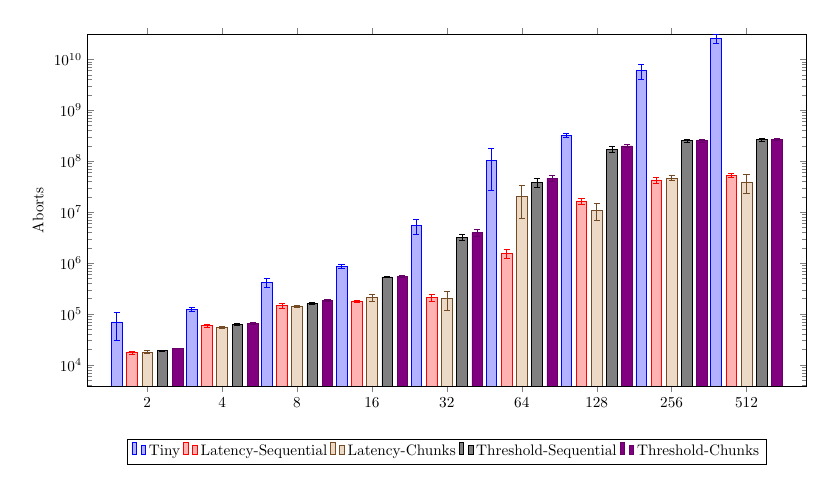
\begin{tikzpicture}[scale=0.55, baseline]
        \begin{axis}[
            ymode=log,
            width=1.5 \linewidth,
            height=0.8 \linewidth,
            %media de tempo intruder
            ybar=3pt,
            %enlargelimits=0.10,
            legend style={at={(0.5,-0.15)}, anchor=north, legend columns=-1},
            ylabel=Aborts,
            symbolic x coords={1, 2, 4, 8, 16, 32, 64, 128, 256, 512},
            xtick=data,
            ymin=0,
            ymax=31000000000,
            bar width=7pt,
            % nodes near coords,
            nodes near coords align={vertical},
        ]
        \addplot+[error bars,y dir=both, y explicit] coordinates {
            (1,0.0)+-(1,0.0) (2,69940.4)+-(2,38859.442881235445) (4,123224.4)+-(4,10230.047558051723) (8,421702.0)+-(8,83144.47432752221) (16,858817.0)+-(16,70319.27963794851) (32,5482927.6)+-(32,1822574.306164838) (64,102125071.2)+-(64,75531726.60526115) (128,324906951.0)+-(128,25833176.356745664) (256,5976414236.0)+-(256,1965369780.1742249) (512,25331573456.2)+-(512,5125278647.27645) 
        };
        \addplot+[error bars,y dir=both, y explicit] coordinates {
            (1,0.0)+-(1,0.0) (2,17295.8)+-(2,884.117051074121) (4,58832.4)+-(4,5182.0950049183775) (8,145328.0)+-(8,14502.15570182585) (16,179942.6)+-(16,9939.803108713975) (32,213282.4)+-(32,33756.78063204487) (64,1563534.8)+-(64,303501.08637854987) (128,16550448.4)+-(128,2123035.5644618487) (256,42956098.2)+-(256,6012180.935710481) (512,52269879.0)+-(512,4755551.76397057)
        };
        \addplot+[error bars,y dir=both, y explicit] coordinates {
             (1,0.0)+-(1,0.0) (2,17786.7)+-(2,1249.259304548099) (4,54750.2)+-(4,2738.370420523856) (8,141273.5)+-(8,6123.819286197136) (16,209526.5)+-(16,34736.26421551402) (32,201599.3)+-(32,81127.76465680539) (64,20569626.4)+-(64,12875680.754533986) (128,10897558.0)+-(128,4040389.7657925775) (256,46668204.777777776)+-(256,5450523.901092766) (512,39389491.0)+-(512,16022591.920577014) 
        };
        \addplot+[error bars,y dir=both, y explicit] coordinates {
            (1,0.0)+-(1,0.0) (2,19074.2)+-(2,369.0059078117856) (4,61648.4)+-(4,2902.3763091646124) (8,161693.8)+-(8,9525.331540686655) (16,536547.4)+-(16,18869.180433712536) (32,3237316.8)+-(32,385306.9331768636) (64,38103581.6)+-(64,7477543.014654762) (128,171013189.4)+-(128,21848968.54501459) (256,256035773.6)+-(256,17482704.25370147) (512,263634097.2)+-(512,12981014.911830684)
        };
        \addplot+[error bars,y dir=both, y explicit] coordinates {
            (1,0.0)+-(1,0.0) (2,21093.1)+-(2,312.0) (4,64726.72)+-(4,3041.77) (8,183647.1)+-(8,8673.62) (16,544787.54)+-(16,23782.8) (32,3980021.4)+-(32,552484.0028907986) (64,45836278.2)+-(64,6287845.41) (128,199521897.4)+-(128,10431600.060439752) (256,254781534.6)+-(256,19017136.502195936) (512,266950650.75)+-(512,14874593.300939599)
        };
        \legend {Tiny, Latency-Sequential, Latency-Chunks, Threshold-Sequential, Threshold-Chunks}
        \end{axis}
        \end{tikzpicture}
    }

    \subfloat[Yada]{
        \label{Yada}
        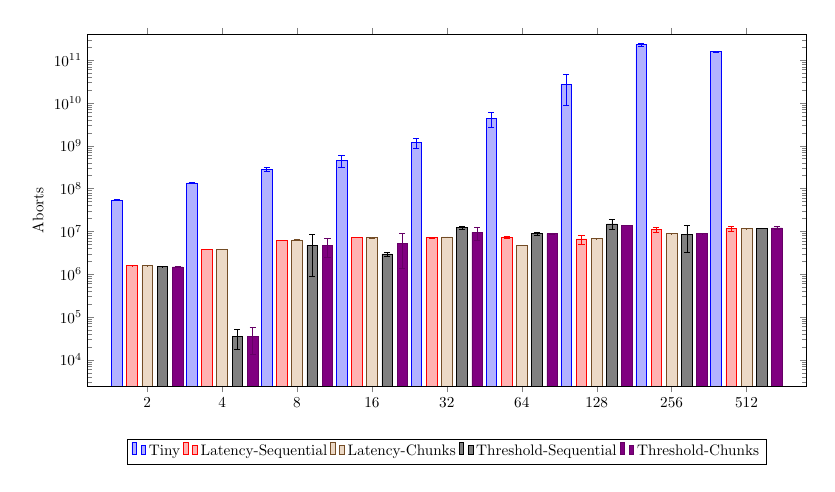
\begin{tikzpicture}[scale=0.55, baseline]
        \begin{axis}[
            ymode=log,
            width=1.5 \linewidth,
            height=0.8 \linewidth,
            %media de tempo intruder
            ybar=3pt,
            %enlargelimits=0.10,
            legend style={at={(0.5,-0.15)}, anchor=north, legend columns=-1},
            ylabel=Aborts,
            symbolic x coords={1, 2, 4, 8, 16, 32, 64, 128, 256, 512},
            xtick=data,
            ymin=0,
            ymax=400000000000,
            bar width=7pt,
            % nodes near coords,
            nodes near coords align={vertical},
        ]
        \addplot+[error bars,y dir=both, y explicit] coordinates {
            (1,0.0)+-(1,0.0) (2,53805739.2)+-(2,945974.4856792702) (4,136025541.2)+-(4,4837342.13) (8,281305083.6)+-(8,28618515.67361887) (16,455944205.2)+-(16,138166587.07) (32,1205121875.2)+-(32,315403375.80832976) (64,4297295036.4)+-(64,1609418223.03) (128,27371816768.6)+-(128,18399453268.002537) (256,230017372308.6)+-(256,19982225506.96) (512,156775482845.2)+-(512,5418181512.20) 
        };
        \addplot+[error bars,y dir=both, y explicit] coordinates {
            (1,0.0)+-(1,0.0) (2,1580633.2)+-(2,8478.500749542929) (4,3800972.6)+-(4,20650.110223434644) (8,6149664.4)+-(8,75882.93103880476) (16,7207458.2)+-(16,106075.91092684522) (32,7097792.4)+-(32,149914.3555148739) (64,7245601.6)+-(64,297306.3815181907) (128,6626592.6)+-(128,1601916.1098185633) (256,11035923.666666666)+-(256,1354186.7993902795) (512,11463741.25)+-(512,1422857.6912357355)
        };
        \addplot+[error bars,y dir=both, y explicit] coordinates {
             (1,0.0)+-(1,0.0) (2,1586885.6)+-(2,17013.20809959133) (4,3864768.25)+-(4,23733.99245149244) (8,6283745.6)+-(8,79485.5) (16,7192878.4)+-(16,178424.65) (32,7378729.9)+-(32,18573.11) (64,4723078.0)+-(64,3928.0) (128,6736182.0)+-(128,37123.3) (256,8828877.0)+-(256,12847.0) (512,11637482.0)+-(512,82034.0) 
        };
        \addplot+[error bars,y dir=both, y explicit] coordinates {
            (1,0.0)+-(1,0.0) (2,1502389.8)+-(2,8336.5398735266599) (4,34570.6)+-(4,17081.853735470282) (8,4673390.0)+-(8,3789634.775837482) (16,2964970.8)+-(16,290439.4272928145) (32,12301780.8)+-(32,1054972.452489657) (64,9002166.4)+-(64,735560.767845634) (128,14938022.8)+-(128,3727246.128412794) (256,8642330.0)+-(256,5465830.0) (512,11928378.731)+-(512,74928.0)
        };
        \addplot+[error bars,y dir=both, y explicit] coordinates {
            (1,0.0)+-(1,0.0) (2,1483981.3)+-(2,5287.71) (4,34983.38)+-(4,21305.7) (8,4728374.12)+-(8,2263748.1) (16,5260517.0)+-(16,3862894.25) (32,9462941.0)+-(32,3192100.38) (64,8837692.27)+-(64,384722.0) (128,13729279.5)+-(128,110344.5) (256,8874348.23)+-(256,63743.0) (512,11973628.0)+-(512,837874.02)
        };
        \legend {Tiny, Latency-Sequential, Latency-Chunks, Threshold-Sequential, Threshold-Chunks}
        \end{axis}
        \end{tikzpicture}
    }
    
    \caption{Aborts em NUMA variando o número de \emph{threads}.}
    \label{abort2}

\end{figure}